\documentclass[tikz,border=10pt]{standalone}
\usepackage{amsmath}
\begin{document}
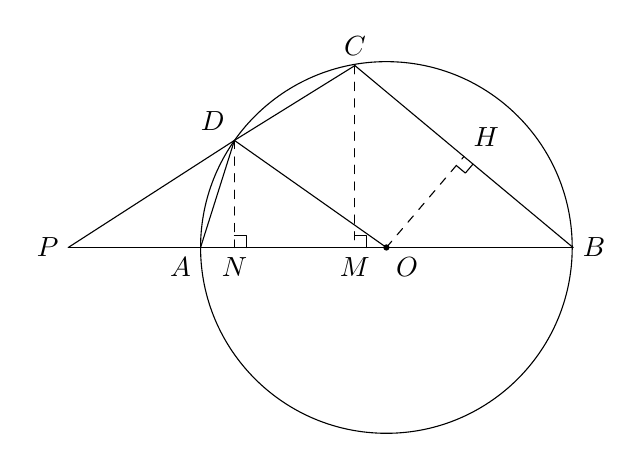
\begin{tikzpicture}[scale=1, line cap=round, line join=round]

% Points
\coordinate (P) at (-4.04,0);
\coordinate (A) at (-2.36,0);
\coordinate (N) at (-1.93,0);
\coordinate (M) at (-0.40,0);
\coordinate (O) at (0,0);
\coordinate (B) at (2.37,0);
\coordinate (C) at (-0.40,2.31);
\coordinate (D) at (-1.93,1.36);
\coordinate (H) at (0.985,1.155);

% Circle
\draw (O) circle (2.36);

% Solid edges
\draw (P) -- (B);
\draw (P) -- (D);
\draw (D) -- (C);
\draw (D) -- (A);
\draw (D) -- (O);
\draw (C) -- (B);

% Dashed edges
\draw[dashed] (C) -- (M);
\draw[dashed] (D) -- (N);
\draw[dashed] (O) -- (H);

% Right angle marks
\draw (N) ++(0,0.15) -- ++(0.15,0) -- ++(0,-0.15);
\draw (M) ++(0,0.15) -- ++(0.15,0) -- ++(0,-0.15);
\draw (0.888,1.041) -- (1.003,0.945) -- (1.100,1.059);

% Points
\fill (O) circle (0.04);

% Labels
\node[above] at (C) {$C$};
\node[above left] at (D) {$D$};
\node[above right] at (H) {$H$};
\node[left] at (P) {$P$};
\node[below left] at (A) {$A$};
\node[below] at (N) {$N$};
\node[below] at (M) {$M$};
\node[below right] at (O) {$O$};
\node[right] at (B) {$B$};

\end{tikzpicture}
\end{document}
